% Provenance (never printed): see sources/outline_sources.md (Year 1: vertical structure of
% the atmosphere, lapse rates, potential temperature and static stability; the layered
% ocean, the equation of state of seawater, T-S diagrams and water masses). Exercise and
% problem values in the Book 3 scratch calculator calc/ch26.py; figures from
% figdata/bachelor-1/atmosphere_profile.py (U.S. Standard Atmosphere 1976) and
% seawater_eos.py (EOS-80 and the UNESCO 44 algorithms; WOA23 columns, datasets
% bachelor-1-woa23-* and Book 2's grade-10-woa23-arctic-*).
% Physics owns the hydrostatic relation, the isothermal atmosphere and its scale height,
% the first law, Laplace's relation and Archimedes' thrust (recalled). Book 1 (g8) gave
% the layers and the environmental lapse rate of 6.5 K/km; Book 2 (g10) the dry adiabatic
% rate admitted, stable and unstable air, the mixed layer, thermocline, halocline and
% pycnocline: re-founded here with derivations. The moist adiabat is the Year 2 volume's.
\chapter{Structure of the Atmosphere and the Ocean}\label{ch:b1:fluid-envelopes-structure}

Twice a day, at weather stations around the world, a balloon is released carrying
a radiosonde, a small instrument that radios back the pressure, the temperature
and the humidity of the air as it rises; it climbs at about \qty{300}{m} a minute
and can pass \qty{35}{km} before the balloon bursts. Far out at sea, a research
ship lowers a frame of instruments and water bottles on a cable to the abyss,
measuring the conductivity, the temperature and the depth all the way. The two
profiles, one of the air and one of the water, are the raw material of this
chapter. Both envelopes are layered, and in both the layering is set by density:
light fluid above heavy fluid. What makes a layer light or heavy is less obvious
than it looks. Air that is colder than the air below it can still be the lighter;
water that is warmer than the water above it can still be the heavier. The
chapter builds the two tools that sort this out, the \omterm{def:b1:fluid-envelopes-structure:potential-temperature}{potential temperature} and
the \omterm{def:b1:fluid-envelopes-structure:eos}{equation of state of seawater}.
% ledger: nws:radiosonde, nws:radiosonde-def, commons:ctd-rosette

\begin{omfigure}
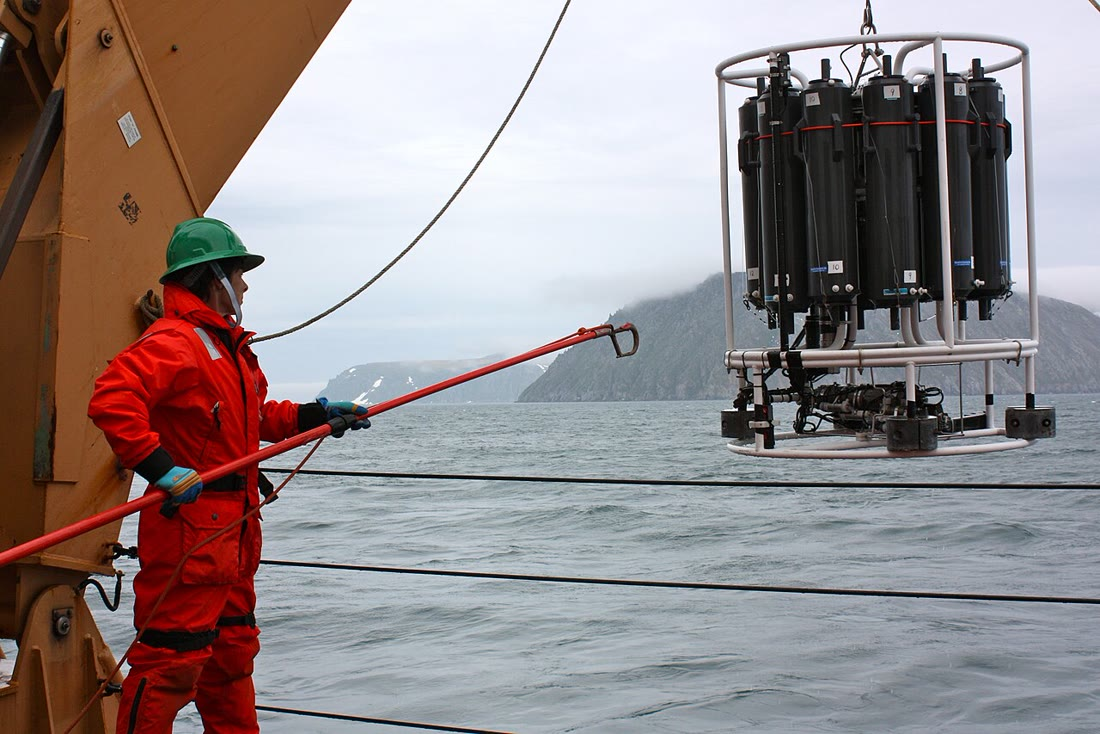
\includegraphics[width=0.62\linewidth]{images/book3/b1-ctd-rosette.jpg}

{\small A CTD and rosette being brought back on board in the Bering Strait in
June 2011. The grey bottles round the frame are closed at chosen depths on the
way up to sample the water; the instruments at the bottom of the frame measure
conductivity (from which salinity is computed), temperature and depth (in fact
pressure) continuously as the frame is lowered. (NASA Goddard Space Flight
Center, public domain, via Wikimedia Commons.)}
\label{fig:b1:fluid-envelopes-structure:ctd}
\end{omfigure}
% ledger: commons:ctd-rosette, unesco44:atg-theta

\begin{recall}
The physics volumes give the hydrostatic relation, $\mathrm dp/\mathrm dz =
-\rho g$, for a fluid at rest; for an ideal gas of molar mass $M$, $p = \rho R
T/M$, and in an isothermal atmosphere the pressure falls as $e^{-z/H}$ with the
scale height $H = RT/(Mg)$. They state the first law for a closed system and,
for an ideal gas, Laplace's relation along a reversible adiabatic
transformation, $pV^{\gamma} = $ constant, with $\gamma = c_p/c_v$ and $c_p - c_v
= R/M$ per unit mass. A body immersed in a fluid receives an upward thrust equal
to the weight of fluid it displaces (Archimedes). Book~1 named the layers of the
atmosphere and the \omterm{def:b1:fluid-envelopes-structure:lapse-rate}{environmental lapse rate} of the \omterm{def:b1:fluid-envelopes-structure:standard-atmosphere}{standard atmosphere},
\qty{6.5}{\celsius} per kilometre in the troposphere; Book~2 admitted the dry
adiabatic rate, \qty{9.8}{\celsius} per kilometre, called air stable or unstable
according to the fate of a parcel pushed upwards, and described the \omterm{def:b1:fluid-envelopes-structure:ocean-layers}{mixed layer},
the \omterm{def:b1:fluid-envelopes-structure:ocean-layers}{thermocline}, the \omterm{def:b1:fluid-envelopes-structure:ocean-layers}{halocline} and the \omterm{def:b1:fluid-envelopes-structure:ocean-layers}{pycnocline} of the ocean. The salinity of
seawater is close to 35 grams of dissolved salts per kilogram.
% ledger: ussa76:layers, nws:dalr, nos:salinity
\end{recall}

\section{The vertical structure of the atmosphere}\label{sec:b1:fluid-envelopes-structure:atmosphere}

No real sounding is the same as the next one. To compare them, a reference
profile is fixed by convention.

\begin{definition}[Standard atmosphere]\label{def:b1:fluid-envelopes-structure:standard-atmosphere}
A \emph{standard atmosphere}\index{standard atmosphere} is a profile of
temperature, pressure and density against height fixed by convention: dry air
of constant molar mass, an ideal gas in hydrostatic balance, with given values at
sea level and a temperature that varies linearly with height in successive
layers. The 1976 standard atmosphere takes \qty{288.15}{K} and
\qty{101325}{Pa} at sea level, $M_0 = \qty{28.9644}{kg.kmol^{-1}}$,
$R^* = \qty{8314.32}{J.kmol^{-1}.K^{-1}}$ and $g_0 = \qty{9.80665}{m.s^{-2}}$.
\end{definition}
% ledger: ussa76:sea-level

Below \qty{47}{km} the 1976 standard has four layers
(\cref{tab:b1:fluid-envelopes-structure:layers}). The lowest, the troposphere,
cools at \qty{6.5}{K} per kilometre; from its top, the tropopause, the
temperature stays at \qty{216.65}{K} for nine kilometres, then rises. The
heights of the standard are geopotential heights, the heights that a constant
gravity $g_0$ would give the same potential energy; below \qty{32}{km} they
differ from geometric heights by less than \qty{0.6}{\percent}
(\qty{11}{km} of the standard lie at \qty{11.02}{km}).
% ledger: ussa76:layers, ussa76:sea-level

\begin{table}[ht]
\centering
\small
\renewcommand{\arraystretch}{1.2}
\begin{tabular}{|l|c|c|c|c|}
\hline
Layer & Base (km) & $\mathrm dT/\mathrm dz$ (K/km) & $T$ at base (K) & $p$ at base (hPa) \\
\hline
1 (troposphere) & 0 & $-6.5$ & 288.15 & 1013.25 \\
2 (stratosphere) & 11 & 0.0 & 216.65 & 226.32 \\
3 (stratosphere) & 20 & $+1.0$ & 216.65 & 54.75 \\
4 (stratosphere) & 32 & $+2.8$ & 228.65 & 8.68 \\
\hline
\end{tabular}
\caption{The four lowest layers of the 1976 \omterm{def:b1:fluid-envelopes-structure:standard-atmosphere}{standard atmosphere}. The gradients
and the sea-level values are defining values; the temperatures and pressures at
the bases are computed from them with \cref{prop:b1:fluid-envelopes-structure:layer-pressure}.}
\label{tab:b1:fluid-envelopes-structure:layers}
\end{table}
% ledger: ussa76:layers, ussa76:sea-level (bases computed in figdata/bachelor-1/atmosphere_profile.py)

In each layer the temperature is a linear function of height, so the
hydrostatic relation can be integrated in closed form.

\begin{proposition}[Pressure in a layer of constant gradient]\label{prop:b1:fluid-envelopes-structure:layer-pressure}
In a layer of dry air where $T = T_b - L\,(z - z_b)$ with a constant $L \neq 0$, the
pressure is
\[
  p = p_b \left(\frac{T}{T_b}\right)^{gM/(RL)},
\]
where $T_b$ and $p_b$ are the values at the base $z_b$. When $L = 0$ the
pressure falls exponentially with the scale height $H = RT_b/(Mg)$.
\end{proposition}

\begin{proof}
The hydrostatic relation and the ideal gas give $\mathrm dp/p = -(gM/R)\,\mathrm
dz/T$. Since $\mathrm dT = -L\,\mathrm dz$, this is $\mathrm dp/p =
(gM/(RL))\,\mathrm dT/T$, which integrates to $\ln(p/p_b) = (gM/(RL))
\ln(T/T_b)$. For $L = 0$, $T = T_b$ and $\ln(p/p_b) = -(z - z_b)/H$: the
isothermal atmosphere of the physics volumes.
\end{proof}

In the troposphere of the standard, $gM/(RL) = 9.80665 \times 28.9644 /
(8314.32 \times 0.0065) = 5.256$, and at \qty{11}{km}, $T = 216.65$~K:
$p = \num{101325} \times (216.65/288.15)^{5.256} = \qty{22632}{Pa}$, a little
under a quarter of the sea-level value. In the isothermal layer above, $H =
8314.32 \times 216.65/(28.9644 \times 9.80665) = \qty{6.34}{km}$, and nine
kilometres higher the pressure has fallen by a further factor $e^{9/6.34} =
4.13$, to \qty{5475}{Pa}. Since the pressure at a level is the weight, per unit
area, of the air above it, half of the mass of the \omterm{def:b1:fluid-envelopes-structure:standard-atmosphere}{standard atmosphere} lies below
\qty{5.5}{km} and nine tenths below \qty{16}{km}.
% ledger: ussa76:sea-level, ussa76:layers (values computed in figdata/bachelor-1/atmosphere_profile.py)

\section{Lapse rates and potential temperature}\label{sec:b1:fluid-envelopes-structure:lapse}

\begin{definition}[Environmental and dry adiabatic lapse rates]\label{def:b1:fluid-envelopes-structure:lapse-rate}
The \emph{environmental lapse rate}\index{environmental lapse rate} is $\Gamma =
-\mathrm dT/\mathrm dz$, the rate at which the temperature of the air at rest
decreases with height, as a sounding measures it. The \emph{dry adiabatic lapse
rate}\index{dry adiabatic lapse rate} $\Gamma_d$ is the rate at which the
temperature of a parcel of unsaturated air decreases as the parcel is lifted.
\end{definition}
% ledger: nws:dalr

A lapse rate is positive when the temperature falls with height. The two rates
are of different natures: the first describes the state of the atmosphere at one
moment; the second, the transformation of a piece of air that moves.

\begin{definition}[Air parcel]\label{def:b1:fluid-envelopes-structure:parcel}
An \emph{air parcel}\index{air parcel} is a volume of air followed in its
motion, small enough to have a single temperature and pressure and not to
disturb the air around it, large enough to keep its identity: it exchanges no
mass and, during a quick displacement, no heat with its surroundings, and its
pressure is at every moment that of the surrounding air.
\end{definition}

The parcel is an idealisation, like the closed system of thermodynamics: the
results below hold for real air to the extent that a moving piece of it exchanges
little heat and little mass with its surroundings.

\begin{theorem}[The dry adiabatic lapse rate]\label{thm:b1:fluid-envelopes-structure:dry-adiabatic}
A parcel of dry air, lifted adiabatically and reversibly through air at rest of
nearly the same temperature, cools at the rate
\[
  \Gamma_d = \frac{g}{c_p},
\]
where $c_p$ is the specific heat of air at constant pressure. With $c_p =
\qty{1004.7}{J.kg^{-1}.K^{-1}}$, $\Gamma_d = \qty{9.76}{K.km^{-1}}$.
\end{theorem}

\begin{proof}
For a kilogram of the parcel, of temperature $T_p$ and density $\rho_p$, the
first law of a reversible transformation without heat exchange, written with the
enthalpy, is $c_p\,\mathrm dT_p - \mathrm dp/\rho_p = 0$. The pressure of the
parcel is that of the air around it, which is hydrostatic: $\mathrm dp = -\rho_e
g\,\mathrm dz$, with $\rho_e$ the density of the surrounding air. Hence
\[
  \frac{\mathrm dT_p}{\mathrm dz} = -\frac{g}{c_p}\,\frac{\rho_e}{\rho_p}
  = -\frac{g}{c_p}\,\frac{T_p}{T_e},
\]
since at equal pressure the densities of two ideal gases of the same molar mass
are in the inverse ratio of their temperatures. When the parcel is at nearly the
temperature of its surroundings, $T_p/T_e \approx 1$ and $-\mathrm dT_p/\mathrm dz
= g/c_p$. For dry air, an ideal diatomic gas, $\gamma = 1.4$, so $c_p =
\gamma/(\gamma - 1) \times R/M = 3.5 \times 8314.32/28.9644 =
\qty{1004.7}{J.kg^{-1}.K^{-1}}$, and $\Gamma_d = 9.80665/1004.7 =
\qty{0.00976}{K.m^{-1}}$.
\end{proof}
% ledger: nasa:grc-gamma, ussa76:sea-level, nws:dalr

A parcel \qty{10}{K} warmer than its surroundings, near \qty{280}{K}, cools at
$\Gamma_d \times 290/280$, \qty{3.6}{\percent} faster; the correction is
neglected in what follows. The rate does not depend on the pressure or the
temperature of the parcel, and a parcel that sinks warms at the same rate, as
Book~2 followed air over a mountain.

Integrating the same equation without the hydrostatic step gives a quantity that
the parcel carries with it.

\begin{proposition}[Potential temperature]\label{prop:b1:fluid-envelopes-structure:theta}
Along a reversible adiabatic transformation of dry air,
\[
  \theta = T\left(\frac{p_0}{p}\right)^{\kappa},\qquad \kappa = \frac{R}{Mc_p} =
  \frac{\gamma - 1}{\gamma} = \frac{2}{7},
\]
stays constant, whatever the reference pressure $p_0$.
\end{proposition}

\begin{proof}
From $c_p\,\mathrm dT = \mathrm dp/\rho$ and $\rho = pM/(RT)$, $c_p\,\mathrm dT/T
= (R/M)\,\mathrm dp/p$, so $\ln T - \kappa \ln p$ is constant, and so is $T
p^{-\kappa}$; multiplying by the constant $p_0^{\kappa}$ gives $\theta$. This is
Laplace's relation written with $T$ and $p$.
\end{proof}

\begin{definition}[Potential temperature]\label{def:b1:fluid-envelopes-structure:potential-temperature}
The \emph{potential temperature}\index{potential temperature} $\theta$ of a
parcel of dry air is the temperature it would have if brought adiabatically to
the reference pressure $p_0 = \qty{1000}{hPa}$: $\theta = T\,(1000/p)^{2/7}$ with
$p$ in hectopascals and $T$ in kelvins.
\end{definition}
% ledger: nws:potential-temperature

The \omterm{def:b1:fluid-envelopes-structure:potential-temperature}{potential temperature} is a label that a dry parcel keeps when it rises or
sinks without exchanging heat, as the salinity of a water parcel is. Heating by
radiation, by condensation of water or by mixing changes it; the rest does not.

\begin{example}[The tropopause of the standard atmosphere]\label{ex:b1:fluid-envelopes-structure:tropopause}
At the surface of the standard, $\theta = 288.15 \times (1000/1013.25)^{2/7} =
\qty{287.07}{K}$. At the tropopause, $T = \qty{216.65}{K}$ and $p =
\qty{226.32}{hPa}$: $\theta = 216.65 \times (1000/226.32)^{2/7} = 216.65 \times
1.529 = \qty{331.2}{K}$. Air from the tropopause brought down adiabatically to
\qty{1000}{hPa} would arrive at \qty{331.2}{K}, \qty{44}{K} warmer than surface
air brought to the same pressure. The temperature falls by \qty{71.5}{K} from
the ground to the tropopause, yet the \omterm{def:b1:fluid-envelopes-structure:potential-temperature}{potential temperature} rises by
\qty{44}{K}.
\end{example}
% ledger: ussa76:layers, nws:potential-temperature (values computed in figdata/bachelor-1/atmosphere_profile.py)

\section{Static stability}\label{sec:b1:fluid-envelopes-structure:stability}

\begin{definition}[Static stability; temperature inversion]\label{def:b1:fluid-envelopes-structure:stability}
The \emph{static stability}\index{static stability} of a layer at rest is its
response to a small vertical displacement of a parcel. The layer has a
\emph{stable stratification}\index{stable stratification} if the displaced
parcel is pushed back towards its level, an \emph{unstable
stratification}\index{unstable stratification} if it is pushed further away,
and a \emph{neutral stratification}\index{neutral stratification} if no force
acts on it. A \emph{temperature inversion}\index{temperature inversion} is a
layer in which the temperature increases with height.
\end{definition}
% ledger: nws:inversion

\begin{theorem}[The criterion of static stability]\label{thm:b1:fluid-envelopes-structure:stability}
A layer of dry air at rest, of temperature $T$ and \omterm{def:b1:fluid-envelopes-structure:lapse-rate}{environmental lapse rate}
$\Gamma$, is stable if $\Gamma < \Gamma_d$, neutral if $\Gamma = \Gamma_d$ and
unstable if $\Gamma > \Gamma_d$; equivalently, it is stable if and only if its
\omterm{def:b1:fluid-envelopes-structure:potential-temperature}{potential temperature} increases with height. A parcel displaced by a small
$\delta z$ in a stable layer oscillates about its level at the
angular frequency $N$, where
\[
  N^2 = \frac{g}{T}\,(\Gamma_d - \Gamma) = \frac{g}{\theta}\,\frac{\mathrm d\theta}{\mathrm dz}.
\]
\end{theorem}

\begin{proof}
A parcel at the temperature $T$ of its level is lifted by $\delta z$. It arrives
at $T - \Gamma_d\,\delta z$, while the air around it is at $T - \Gamma\,\delta z$.
Per unit mass, the parcel feels its weight and the thrust of Archimedes, a net
upward acceleration $g\,(\rho_e - \rho_p)/\rho_p = g\,(T_p - T_e)/T_e$, the
pressures being equal. To first order in $\delta z$ this is
\[
  \frac{\mathrm d^2 \delta z}{\mathrm dt^2} = -\frac{g}{T}\,(\Gamma_d - \Gamma)\,\delta z = -N^2\,\delta z .
\]
If $\Gamma < \Gamma_d$, $N^2 > 0$ and the parcel oscillates at the angular
frequency $N$; if $\Gamma > \Gamma_d$ the displacement grows exponentially; if
$\Gamma = \Gamma_d$ no force acts. For the second form, take the logarithmic
derivative of $\theta = T (p_0/p)^{\kappa}$ and use the hydrostatic relation:
\[
  \frac{1}{\theta}\frac{\mathrm d\theta}{\mathrm dz} = \frac{1}{T}\frac{\mathrm dT}{\mathrm dz}
  - \frac{\kappa}{p}\frac{\mathrm dp}{\mathrm dz} = -\frac{\Gamma}{T} + \frac{\kappa\,\rho g}{p}
  = -\frac{\Gamma}{T} + \frac{\kappa g M}{RT} = \frac{\Gamma_d - \Gamma}{T},
\]
since $\kappa M/R = 1/c_p$.
\end{proof}

The angular frequency $N$ is called the buoyancy frequency. In the troposphere
of the standard, near the ground, $N^2 = (9.80665/288.15) \times (9.761 -
6.5)\times10^{-3} = \qty{1.11e-4}{s^{-2}}$, $N = \qty{0.0105}{s^{-1}}$, and the
period $2\pi/N$ of the oscillation is about \qty{10}{min}. In the isothermal
lower stratosphere $\Gamma = 0$: $N = \qty{0.0210}{s^{-1}}$, twice as large, a
period of five minutes. The stratosphere is a lid: it resists vertical motion
much more strongly than the troposphere below it.
% ledger: ussa76:layers (values computed in figdata/bachelor-1/atmosphere_profile.py)

\begin{omfigure}
\begin{tikzpicture}
\begin{axis}[name=tz, omrecord, width=0.46\linewidth, height=7.2cm, xmin=160, xmax=300,
  ymin=0, ymax=32, xlabel={temperature (K)}, ylabel={height (km)}, xtick={160,200,...,300},
  ytick={0,5,...,30}]
% figdata/bachelor-1/atmosphere_profile.py; ledger: ussa76:sea-level, ussa76:layers, nasa:grc-gamma
\addplot[omDef, line width=0.9pt] table[x=T_K, y=z_km] {figdata/out/bachelor-1-atmosphere_profile-profile.dat};
\addplot[omThm, dashed, line width=0.7pt] table[x=T_K, y=z_km] {figdata/out/bachelor-1-atmosphere_profile-adiabat.dat};
\addplot[only marks, mark=*, mark size=1.6pt, black] table[x=T_K, y=z_km] {figdata/out/bachelor-1-atmosphere_profile-tropo.dat};
\node[font=\scriptsize, text=omThm, anchor=west, align=left] at (axis cs:163,17.0) {dry adiabat\\from the surface};
\node[font=\scriptsize, text=omDef, anchor=west] at (axis cs:252,6.4) {standard};
\node[font=\scriptsize, anchor=east] at (axis cs:214.5,11.9) {tropopause};
\end{axis}
\begin{axis}[at={(tz.east)}, anchor=west, xshift=1.3cm, omrecord, width=0.46\linewidth, height=7.2cm,
  xmin=250, xmax=900, ymin=0, ymax=32, xlabel={potential temperature (K)}, ylabel={height (km)},
  xtick={300,500,700,900}, ytick={0,5,...,30}]
\addplot[omDef, line width=0.9pt] table[x=theta_K, y=z_km] {figdata/out/bachelor-1-atmosphere_profile-profile.dat};
\addplot[only marks, mark=*, mark size=1.6pt, black] table[x=theta_K, y=z_km] {figdata/out/bachelor-1-atmosphere_profile-tropo.dat};
\node[font=\scriptsize, anchor=west] at (axis cs:345,10.2) {\num{331} K};
\end{axis}
\end{tikzpicture}

{\small The 1976 \omterm{def:b1:fluid-envelopes-structure:standard-atmosphere}{standard atmosphere} to \qty{32}{km}. Left: temperature, with
the dry adiabat that a parcel lifted from the surface would follow (dashed). The
standard cools more slowly than the adiabat, so it is stable everywhere. Right:
\omterm{def:b1:fluid-envelopes-structure:potential-temperature}{potential temperature}, which rises with height throughout, gently in the
troposphere and steeply above the tropopause (dot).}
\label{fig:b1:fluid-envelopes-structure:theta}
\end{omfigure}
% ledger: ussa76:sea-level, ussa76:layers, nasa:grc-gamma, nws:potential-temperature

On a diagram of temperature against height, the criterion compares two slopes
(figure below): the parcel follows the dry adiabat through its starting point,
and the question is on which side of the sounding it finds itself after a small
displacement.

\begin{omfigure}
\begin{tikzpicture}[x=0.55cm, y=0.55cm, >={Stealth[length=2mm]}]
\foreach \dx/\envtop/\verdict in {0/-0.8/{stable layer: the parcel sinks back}, 9/-3.8/{unstable layer: the parcel rises on}} {
  \begin{scope}[xshift=\dx cm]
  \draw[->] (0,0) -- (7.2,0) node[below left, font=\scriptsize] {temperature};
  \draw[->] (0,0) -- (0,6.4) node[above right, font=\scriptsize] {height};
  % sounding (environment): solid; dry adiabat through the starting point P: dashed
  \draw[omDef, line width=0.9pt] (5.0,0.6) -- (5.0+\envtop,5.4);
  \draw[omThm, dashed, line width=0.8pt] (5.0,0.6) -- (2.6,5.4);
  \fill (5.0,0.6) circle (2pt) node[right, font=\scriptsize] {$P$};
  \draw[densely dotted] (0,4.2) node[left, font=\scriptsize] {$z + \delta z$} -- (7,4.2);
  \fill[omThm] (3.2,4.2) circle (1.8pt);
  \fill[omDef] ({5.0+\envtop*3.6/4.8},4.2) circle (1.8pt);
  \node[font=\scriptsize, anchor=north] at (3.6,-0.5) {\verdict};
  \end{scope}
}
\end{tikzpicture}

{\small The parcel method. Solid blue: the sounding; dashed red: the dry
adiabat through $P$. A parcel starts at $P$ at the temperature of the air around
it and is lifted to $z + \delta z$ along the dry adiabat (red dot); the sounding
gives the temperature of the air there (blue dot). Left: the sounding
cools more slowly than the adiabat; the parcel arrives colder, hence denser, than
its surroundings and sinks back. Right: the sounding cools faster than the
adiabat; the parcel arrives warmer and keeps rising.}
\label{fig:b1:fluid-envelopes-structure:parcel}
\end{omfigure}

\begin{method}[Reading the stability of a sounding]\label{met:b1:fluid-envelopes-structure:sounding}
\begin{enumerate}
  \item Divide the sounding into layers between levels where the slope changes.
  \item In each layer compute $\Gamma = -(T_2 - T_1)/(z_2 - z_1)$, in kelvins per
        kilometre.
  \item Compare with $\Gamma_d = \qty{9.8}{K/km}$: $\Gamma > \Gamma_d$ unstable,
        $\Gamma$ close to $\Gamma_d$ neutral, $\Gamma < \Gamma_d$ stable; a
        negative $\Gamma$ is an inversion, the most stable case.
  \item Where pressures are given rather than heights, compute $\theta =
        T(1000/p)^{2/7}$ at each level: $\theta$ decreasing upwards marks an
        unstable layer, constant a neutral one, increasing a stable one.
\end{enumerate}
\end{method}

An unstable layer does not last: a displacement in it grows exponentially, at
the rate $\sqrt{-N^2}$, and the parcels it releases overturn it, mixing it until
its \omterm{def:b1:fluid-envelopes-structure:potential-temperature}{potential temperature} is uniform and its lapse rate is $\Gamma_d$. A layer
heated from below, by warm ground or a warm sea, is pushed towards instability;
one cooled from below, towards stability. An inversion caps whatever lies below
it: a parcel rising from below finds itself colder than its surroundings as soon
as it enters it. Above \qty{20}{km} the whole stratosphere of the standard is an
inversion.

All of this assumes dry air. A rising parcel that becomes saturated releases
latent heat as its water condenses and cools more slowly than $\Gamma_d$; the
saturated adiabat and the conditional instability it brings are the subject of
next year's volume.
% ledger: nws:inversion, nws:dalr

\section{The layered ocean}\label{sec:b1:fluid-envelopes-structure:ocean}

The ocean exchanges heat and water with the atmosphere only at its surface,
through heating and cooling, evaporation and rain. Its vertical structure has
three ingredients, temperature, salinity and density.

\begin{definition}[Mixed layer, thermocline, halocline, pycnocline]\label{def:b1:fluid-envelopes-structure:ocean-layers}
The \emph{mixed layer}\index{mixed layer} is the surface layer of the ocean
whose temperature, salinity and density are nearly uniform with depth; its
depth is read on a profile as the depth where the temperature first differs from
its surface value by a chosen threshold, often \qty{0.5}{\celsius}. The
\emph{thermocline}\index{thermocline}, the \emph{halocline}\index{halocline} and
the \emph{pycnocline}\index{pycnocline} are the layers below it in which the
temperature, the salinity and the density respectively change fastest with
depth.
\end{definition}

The pressure in the ocean is quoted in decibars, because one decibar,
\qty{e4}{Pa}, is nearly the pressure of one metre of seawater: at
\qty{30}{\degree} of \omterm{def:b1:spherical-astronomy:geographic}{latitude}, \qty{1000}{dbar} lie at \qty{990.8}{m} and
\qty{10000}{dbar} at \qty{9712.7}{m}.
% ledger: unesco:eos80-checks (DEPTH table computed in figdata/bachelor-1/seawater_eos.py)

Water is nearly incompressible, but not quite, and a parcel of water brought
up from the deep expands and cools a little, as a parcel of air does. The
adiabatic lapse rate of seawater is small, about \qty{0.04}{\celsius} per
\qty{1000}{dbar} at the surface at \qty{0}{\celsius} and \qty{0.09}{\celsius}
per \qty{1000}{dbar} at \qty{3000}{dbar}, against \num{9.8} per kilometre in
air; but over five kilometres it adds up to a few tenths of a degree, more than
the differences between deep waters. Oceanographers therefore compare waters by
their \emph{potential} temperature too: the temperature a parcel would have if
raised adiabatically, without change of salinity, to the surface. A water of
\qty{2}{\celsius} at \qty{4000}{dbar} and salinity 35 has a \omterm{def:b1:fluid-envelopes-structure:potential-temperature}{potential
temperature} of \qty{1.66}{\celsius}. In the deepest levels of the South
Atlantic at \qty{10.5}{\degree S}, the measured temperature rises from
\qty{0.730}{\celsius} at \qty{5400}{m} to \qty{0.731}{\celsius} at \qty{5500}{m}
while the \omterm{def:b1:fluid-envelopes-structure:potential-temperature}{potential temperature} falls from \qty{0.261}{\celsius} to
\qty{0.250}{\celsius}: the warming is compression, not heat.
% ledger: unesco44:atg-theta, data:b3-woa23 (values computed in figdata/bachelor-1/seawater_eos.py)

\begin{omfigure}
\begin{tikzpicture}
\begin{groupplot}[group style={group size=3 by 1, horizontal sep=0.55cm, yticklabels at=edge left},
  omrecord, omdepth, width=0.365\linewidth, height=7.4cm, ymin=0, ymax=2000,
  ytick={0,500,1000,1500,2000}, y tick label style={/pgf/number format/.cd, set thousands separator={}},
  every axis label/.append style={font=\small}]
\nextgroupplot[xmin=-2, xmax=28, xlabel={$\theta$ (\si{\celsius})}, ylabel={depth (m)}, xtick={0,10,20}]
% figdata/bachelor-1/seawater_eos.py; WOA23 (datasets bachelor-1-woa23-*, grade-10-woa23-arctic-*); ledger: data:b3-woa23, data:b2-woa23, unesco44:atg-theta
\addplot[omThm, line width=0.8pt] table[x=theta, y=depth] {figdata/out/bachelor-1-seawater_eos-prof-sa10.dat};
\addplot[omProp, line width=0.8pt] table[x=theta, y=depth] {figdata/out/bachelor-1-seawater_eos-prof-sa30.dat};
\addplot[omDef, line width=0.8pt] table[x=theta, y=depth] {figdata/out/bachelor-1-seawater_eos-prof-arctic.dat};
\draw[omThm, line width=0.8pt] (axis cs:9,1250) -- (axis cs:13,1250) node[right, font=\scriptsize, text=black] {\qty{10.5}{\degree S}};
\draw[omProp, line width=0.8pt] (axis cs:9,1450) -- (axis cs:13,1450) node[right, font=\scriptsize, text=black] {\qty{30.5}{\degree S}};
\draw[omDef, line width=0.8pt] (axis cs:9,1650) -- (axis cs:13,1650) node[right, font=\scriptsize, text=black] {\qty{75.5}{\degree N}};
\nextgroupplot[xmin=28, xmax=37.5, xlabel={salinity}, xtick={28,31,34,37}]
\addplot[omThm, line width=0.8pt] table[x=s, y=depth] {figdata/out/bachelor-1-seawater_eos-prof-sa10.dat};
\addplot[omProp, line width=0.8pt] table[x=s, y=depth] {figdata/out/bachelor-1-seawater_eos-prof-sa30.dat};
\addplot[omDef, line width=0.8pt] table[x=s, y=depth] {figdata/out/bachelor-1-seawater_eos-prof-arctic.dat};
\nextgroupplot[xmin=22, xmax=28.5, xlabel={$\sigma_\theta$ (\si{kg.m^{-3}})}, xtick={22,24,26,28}]
\addplot[omThm, line width=0.8pt] table[x=sigma, y=depth] {figdata/out/bachelor-1-seawater_eos-prof-sa10.dat};
\addplot[omProp, line width=0.8pt] table[x=sigma, y=depth] {figdata/out/bachelor-1-seawater_eos-prof-sa30.dat};
\addplot[omDef, line width=0.8pt] table[x=sigma, y=depth] {figdata/out/bachelor-1-seawater_eos-prof-arctic.dat};
\end{groupplot}
\end{tikzpicture}

{\small \omterm{def:b1:fluid-envelopes-structure:potential-temperature}{Potential temperature}, salinity and potential \omterm{def:b1:fluid-envelopes-structure:eos}{density anomaly}
(\cref{def:b1:fluid-envelopes-structure:eos}) in the upper \qty{2000}{m}, in the
annual mean, at three places: the tropical South Atlantic (\qty{10.5}{\degree
S}, \qty{25.5}{\degree W}), the subtropical South Atlantic (\qty{30.5}{\degree
S}, \qty{25.5}{\degree W}) and the Canada Basin of the Arctic Ocean
(\qty{75.5}{\degree N}, \qty{150.5}{\degree W}). Data: World Ocean Atlas 2023.}
\label{fig:b1:fluid-envelopes-structure:profiles}
\end{omfigure}
% ledger: data:b3-woa23, data:b2-woa23, unesco:eos80, unesco44:atg-theta

The three columns of the figure above show the three kinds of upper ocean. In
the tropics, a warm \omterm{def:b1:fluid-envelopes-structure:ocean-layers}{mixed layer} near \qty{26.5}{\celsius} sits on a sharp
\omterm{def:b1:fluid-envelopes-structure:ocean-layers}{thermocline}: between \qty{100}{m} and \qty{200}{m} the \omterm{def:b1:fluid-envelopes-structure:potential-temperature}{potential temperature}
drops from \qty{24.0}{\celsius} to \qty{14.4}{\celsius}, and the density follows
it, so the \omterm{def:b1:fluid-envelopes-structure:ocean-layers}{thermocline} is also the \omterm{def:b1:fluid-envelopes-structure:ocean-layers}{pycnocline}. At \qty{30.5}{\degree S} the
surface is cooler, \qty{21.1}{\celsius}, and the fall more gradual, spread over
the upper \qty{800}{m}. In both, salinity is highest near the surface and
decreases downwards; it works against the stratification, which the temperature
more than makes up for. The Arctic column
is the opposite case. Its surface water, at \qty{-1.4}{\celsius}, is the coldest
of the three, yet the lightest, $\sigma_\theta = 22.5$, because its salinity is
only \num{28.1}; salinity rises to \num{34.5} at \qty{300}{m}. The \omterm{def:b1:fluid-envelopes-structure:ocean-layers}{halocline} is
the \omterm{def:b1:fluid-envelopes-structure:ocean-layers}{pycnocline} here. Below it lies a layer warmer than the water above, near
\qty{0.7}{\celsius} at \qty{475}{m}: a \omterm{def:b1:fluid-envelopes-structure:stability}{temperature inversion} that is perfectly
stable, held down by its salt.
% ledger: data:b3-woa23, data:b2-woa23 (values computed in figdata/bachelor-1/seawater_eos.py)

\section{Seawater density and T--S diagrams}\label{sec:b1:fluid-envelopes-structure:ts}

\begin{definition}[Equation of state of seawater; haline contraction coefficient; density anomaly]\label{def:b1:fluid-envelopes-structure:eos}
The \emph{equation of state of seawater}\index{equation of state of seawater}
gives its density $\rho(S, T, p)$ as a function of salinity, temperature and
pressure. The \emph{haline contraction coefficient}\index{haline contraction
coefficient} is $\beta = (1/\rho)\,\partial\rho/\partial S$ at constant
temperature and pressure. The \emph{density anomaly}\index{density anomaly}
$\sigma$ is a density minus \qty{1000}{kg.m^{-3}}: $\sigma_t = \rho(S, T, 0) -
1000$ uses the measured temperature at zero sea pressure, and the potential
density anomaly $\sigma_\theta = \rho(S, \theta, 0) - 1000$ the \omterm{def:b1:fluid-envelopes-structure:potential-temperature}{potential
temperature}.
\end{definition}
% ledger: teos10:alpha-beta, teos10:sigma

The equation of state is not derived from first principles but fitted to
laboratory measurements. The international equation of 1980 at the pressure of
the surface is a polynomial with fifteen coefficients, $\rho = \rho_w(T) +
A(T)\,S + B(T)\,S^{3/2} + C\,S^2$, where $\rho_w$ is the density of pure water;
it gives $\rho(35, \qty{0}{\celsius}) = \qty{1028.1063}{kg.m^{-3}}$. A
thermodynamic description of seawater, TEOS-10, was adopted in 2009 to replace
it as the official one; the 1980 equation is used here because its polynomial
fits on a page. Its thermal
expansion coefficient $\alpha = -(1/\rho)\,\partial\rho/\partial T$ is the
coefficient of the physics volumes.
% ledger: unesco:eos80, teos10:alpha-beta, teos10:replaced

\begin{table}[ht]
\centering
\small
\renewcommand{\arraystretch}{1.2}
\begin{tabular}{|c|c|c|c|}
\hline
$T$ (\si{\celsius}) & $\rho(35, T, 0)$ (\si{kg.m^{-3}}) & $\alpha$ (\si{K^{-1}}) & $\beta$ \\
\hline
0 & 1028.106 & \num{0.53e-4} & \num{7.85e-4} \\
10 & 1026.952 & \num{1.67e-4} & \num{7.61e-4} \\
25 & 1023.343 & \num{2.97e-4} & \num{7.39e-4} \\
\hline
\end{tabular}
\caption{Density and expansion coefficients of seawater of salinity 35 at the
surface pressure, from the international equation of state of 1980.}
\label{tab:b1:fluid-envelopes-structure:density}
\end{table}
% ledger: unesco:eos80 (computed in figdata/bachelor-1/seawater_eos.py)

The expansion coefficient is six times larger in warm water than in water near
freezing, while $\beta$ hardly changes (\cref{tab:b1:fluid-envelopes-structure:density}).
One unit of salinity weighs as much as about \qty{4.6}{\celsius} at
\qty{10}{\celsius}, but as much as \qty{15}{\celsius} near \qty{0}{\celsius}: in
cold polar water, density is set by salinity, as the Arctic column showed.

\begin{proposition}[Linear equation of state]\label{prop:b1:fluid-envelopes-structure:linear-eos}
Near a reference state $(S_0, T_0)$ of density $\rho_0$, at fixed pressure,
\[
  \rho \approx \rho_0\bigl[1 - \alpha\,(T - T_0) + \beta\,(S - S_0)\bigr],
\]
with $\alpha$ and $\beta$ evaluated at the reference state; the error is of second
order in $T - T_0$ and $S - S_0$.
\end{proposition}

\begin{proof}
This is the first-order Taylor expansion of $\rho(S, T)$ at $(S_0, T_0)$, since
$\partial\rho/\partial T = -\rho_0\alpha$ and $\partial\rho/\partial S =
\rho_0\beta$ there.
\end{proof}

About $(35, \qty{10}{\celsius})$ the linear form gives the density of water at
$(35.2, \qty{11}{\celsius})$ within \qty{0.01}{kg.m^{-3}}, but that of a surface
water at $(35.8, \qty{22.4}{\celsius})$ \qty{0.74}{kg.m^{-3}} too high: the
equation of state is curved, and its curvature has consequences.
% ledger: unesco:eos80 (computed in calc/ch26.py)

\begin{definition}[T--S diagram; water mass]\label{def:b1:fluid-envelopes-structure:ts-diagram}
A \emph{T--S diagram}\index{T--S diagram} is a plot of the \omterm{def:b1:fluid-envelopes-structure:potential-temperature}{potential
temperature} of the samples of a profile against their salinity, with the depths
written along the curve and the lines of equal $\sigma_\theta$ drawn underneath.
A \emph{water mass}\index{water mass} is a body of water with a common formation
history, recognised by its range of \omterm{def:b1:fluid-envelopes-structure:potential-temperature}{potential temperature} and salinity.
\end{definition}
% ledger: tomczak:water-masses

A \omterm{def:b1:fluid-envelopes-structure:ts-diagram}{water mass} acquires its temperature and salinity at the surface, through
heating and cooling, evaporation and rain, in the region where it forms; once it
sinks below the \omterm{def:b1:fluid-envelopes-structure:ocean-layers}{mixed layer}, out of contact with the atmosphere, it can change
them only by mixing with its neighbours. \omterm{def:b1:fluid-envelopes-structure:potential-temperature}{Potential temperature} and salinity are
then tracers.

\begin{proposition}[Mixing lines are straight]\label{prop:b1:fluid-envelopes-structure:mixing}
When masses $m_1$ and $m_2$ of two waters $(S_1, \theta_1)$ and $(S_2, \theta_2)$
mix completely, the mixture has
\[
  S = \frac{m_1 S_1 + m_2 S_2}{m_1 + m_2},\qquad
  \theta \approx \frac{m_1 \theta_1 + m_2 \theta_2}{m_1 + m_2}:
\]
on a \omterm{def:b1:fluid-envelopes-structure:ts-diagram}{T--S diagram} it lies on the segment joining the two waters, at distances
from them in the inverse ratio of their masses. Mixtures of three waters fill the
triangle they form.
\end{proposition}

\begin{proof}
The salinity is a mass fraction of salt, and salt is conserved: the mass of salt
in the mixture, $m_1 S_1 + m_2 S_2$, divided by its mass, gives $S$. Mixing at
constant pressure conserves the enthalpy; with a specific heat that varies
little, this is a weighted mean of the \omterm{def:b1:fluid-envelopes-structure:potential-temperature}{potential temperatures}, to within a
relative error of about $3.4\times10^{-4}$ per unit of salinity difference. The
point $(S, \theta)$ is then the barycentre of the two points with the weights
$m_1$ and $m_2$.
\end{proof}
% ledger: teos10:mixing

\begin{omfigure}
\begin{tikzpicture}
\begin{axis}[omrecord, width=0.82\linewidth, height=9cm, xmin=33.5, xmax=37.4, ymin=-2, ymax=28,
  xlabel={salinity}, ylabel={potential temperature (\si{\celsius})}, xtick={34,35,36,37},
  ytick={0,5,...,25}, x tick label style={/pgf/number format/.cd, fixed, precision=1}]
% figdata/bachelor-1/seawater_eos.py; ledger: unesco:eos80, unesco44:atg-theta, data:b3-woa23, tomczak:water-masses
\foreach \s in {24,25,26,26.5,27,27.5,28} {
  \addplot[black!35, line width=0.4pt] table[x=s, y=theta] {figdata/out/bachelor-1-seawater_eos-iso-\s.dat};
}
\addplot[only marks, mark=none, nodes near coords, point meta=explicit symbolic,
  every node near coord/.style={font=\scriptsize, text=black!55, anchor=west}]
  table[x=s, y=theta, meta=lab] {figdata/out/bachelor-1-seawater_eos-isolab.dat};
\addplot[omThm, line width=0.9pt] table[x=s, y=theta] {figdata/out/bachelor-1-seawater_eos-ts-sa10.dat};
\addplot[omProp, line width=0.9pt] table[x=s, y=theta] {figdata/out/bachelor-1-seawater_eos-ts-sa30.dat};
\addplot[only marks, mark=*, mark size=1.7pt, black] table[x=s, y=theta] {figdata/out/bachelor-1-seawater_eos-masses.dat};
\node[font=\scriptsize, anchor=south east] at (axis cs:35.5,15.6) {Central Water};
\node[font=\scriptsize, anchor=south east] at (axis cs:34.25,5.0) {AAIW};
\node[font=\scriptsize, anchor=west] at (axis cs:34.96,2.9) {NADW};
\node[font=\scriptsize, anchor=north] at (axis cs:34.70,0.5) {AABW};
\addplot[omDef, densely dashed, line width=0.7pt, mark=o, mark size=1.8pt] table[x=s, y=theta] {figdata/out/bachelor-1-seawater_eos-cabbeling.dat};
\node[font=\scriptsize, text=omDef, anchor=west] at (axis cs:34.98,7.6) {mixture};
\draw[omThm, line width=0.9pt] (axis cs:33.65,26.2) -- (axis cs:33.95,26.2) node[right, font=\scriptsize, text=black] {\qty{10.5}{\degree S}};
\draw[omProp, line width=0.9pt] (axis cs:33.65,24.7) -- (axis cs:33.95,24.7) node[right, font=\scriptsize, text=black] {\qty{30.5}{\degree S}};
\end{axis}
\end{tikzpicture}

{\small \omterm{def:b1:fluid-envelopes-structure:ts-diagram}{T--S diagram} of the two South Atlantic columns of the profiles figure,
from the surface to the sea floor, over lines of equal potential \omterm{def:b1:fluid-envelopes-structure:eos}{density
anomaly} $\sigma_\theta$ (grey, labelled in \si{kg.m^{-3}} at their upper ends).
Dots: the cores of the water masses read on the column at \qty{30.5}{\degree
S}. Blue: two waters of equal density, $\sigma_\theta = 27.0$, at
\qty{2}{\celsius} and \qty{14}{\celsius}, and their equal-parts mixture, on the
straight line between them and denser than either. Data: World Ocean Atlas
2023.}
\label{fig:b1:fluid-envelopes-structure:ts}
\end{omfigure}
% ledger: data:b3-woa23, unesco:eos80, unesco44:atg-theta, tomczak:water-masses

The two South Atlantic columns draw the same figure on the \omterm{def:b1:fluid-envelopes-structure:ts-diagram}{T--S diagram}: the
similarity of curves from places far apart is what reveals water masses. From
the surface down to about \qty{500}{m}, the curves follow a nearly straight
line, steep in temperature: this is Central Water, which fills the upper
kilometre of the subtropical ocean. Below it, both curves turn to a salinity
minimum, \num{34.30} at \qty{900}{m} and \qty{4.3}{\celsius} at
\qty{30.5}{\degree S}: Antarctic Intermediate Water (AAIW), formed under the
rainy westerlies of the Southern Ocean, sinking to about \qty{1000}{m} and
spreading north. Deeper, a salinity maximum, \num{34.90} at \qty{2900}{m}: North
Atlantic Deep Water (NADW), formed in the Greenland and Labrador Seas, sinking to
about \qty{3000}{m} and moving south through the whole Atlantic. At the bottom
the curves converge on the coldest water, \qty{0.8}{\celsius} at
\qty{4900}{m}: Antarctic Bottom Water (AABW), formed along the Antarctic
continent, which fills the oceans below about \qty{4000}{m}. At
\qty{10.5}{\degree S} the salinity minimum lies at \qty{750}{m} and the maximum
at \qty{1800}{m}, with a higher maximum, \num{34.95}: the NADW is closer to its
source there.
% ledger: tomczak:water-masses, data:b3-woa23 (cores computed in figdata/bachelor-1/seawater_eos.py)

The extremes are themselves mixing products. AAIW, as it moves north, mixes
with the saltier water above and below it; by \cref{prop:b1:fluid-envelopes-structure:mixing}
its core moves towards them on the diagram and the minimum erodes. A salinity
minimum or maximum on a profile is always the trace of a water that came from
elsewhere, carried sideways at its own density level.
% ledger: tomczak:water-masses

\begin{method}[Reading water masses on a T--S diagram]\label{met:b1:fluid-envelopes-structure:ts}
\begin{enumerate}
  \item Convert the measured temperatures to \omterm{def:b1:fluid-envelopes-structure:potential-temperature}{potential temperatures} (in the upper
        kilometre the difference is below \qty{0.1}{\celsius} and may be
        neglected).
  \item Plot $\theta$ against $S$, writing the depths along the curve.
  \item Read the straight segments as mixtures of the two waters at their ends,
        the extremes of salinity or temperature as the cores of water masses,
        and the end of the curve near the bottom as the densest water present.
  \item Read the density on the isopycnals: along a stable profile,
        $\sigma_\theta$ increases with depth.
\end{enumerate}
\end{method}

Because the isopycnals are curved, two waters of the same density do not mix to
a water of that density. Water at $(33.79, \qty{2}{\celsius})$ and water at
$(36.05, \qty{14}{\celsius})$ both have $\sigma_\theta = 27.00$; mixed in equal
parts, they give $(34.92, \qty{8}{\celsius})$, of $\sigma_\theta = 27.21$
(figure above). The mixture is denser than both parents and sinks below them.
This densification on mixing, called cabbeling, is the cost of the curvature of
the equation of state: with the linear form of
\cref{prop:b1:fluid-envelopes-structure:linear-eos}, the density of a mixture
would be the mean of the densities. Along the isopycnal surfaces of the ocean,
where eddies stir waters of different temperature and salinity, cabbeling drives
a slow sinking across them.
% ledger: teos10:cabbeling, unesco:eos80 (example computed in figdata/bachelor-1/seawater_eos.py)

A last caution. Referred to the surface, the AABW at \qty{30.5}{\degree S} comes
out at $\sigma_\theta = 27.854$, slightly lighter than the NADW above it,
\num{27.857}; at the bottom of the column at \qty{10.5}{\degree S}, $\sigma_\theta$
even decreases downwards. The ratio $\alpha/\beta$ of the equation of state
changes with pressure, so that the order of two waters of different temperatures
can depend on the pressure at which their densities are compared. Waters
thousands of metres deep are compared with a density referred to a pressure
nearer their own, such as $\sigma_2$, referred to \qty{2000}{dbar}; the method
is that of next year's volume.
% ledger: teos10:sigma, teos10:thermobaric, data:b3-woa23 (values computed in figdata/bachelor-1/seawater_eos.py)

\section{Exercises}

\begin{exercise}[$\star$]\label{exo:b1:fluid-envelopes-structure:1}
(a)~Compute the scale height of air at \qty{250}{K} with the constants of the
\omterm{def:b1:fluid-envelopes-structure:standard-atmosphere}{standard atmosphere}. (b)~By what factor does the pressure fall over \qty{10}{km}
in an isothermal layer at that temperature? (c)~Why is the scale height smaller
at the tropopause than at the ground?
% ledger: ussa76:sea-level
\end{exercise}

\begin{exercise}[$\star$]\label{exo:b1:fluid-envelopes-structure:2}
A sounding gives, in kelvins per kilometre, the lapse rates $\Gamma = 11.0$
(\qtyrange{0}{0.3}{km}), $9.7$ (\qtyrange{0.3}{1.2}{km}), $-4.0$
(\qtyrange{1.2}{1.5}{km}), $6.0$ (\qtyrange{1.5}{8}{km}) and $0.0$ (above
\qty{8}{km}). Classify each layer as unstable, neutral, stable or an inversion,
and say which is the most stable.
% ledger: nws:dalr, nws:inversion
\end{exercise}

\begin{exercise}[$\star$]\label{exo:b1:fluid-envelopes-structure:3}
(a)~Seawater has a density of \qty{1026.95}{kg.m^{-3}}. What is its \omterm{def:b1:fluid-envelopes-structure:eos}{density
anomaly}? (b)~Of two waters, A with $\sigma_\theta = 27.12$ and B with
$\sigma_\theta = 26.78$, which lies above the other when both are at rest in the
same column? (c)~Why do oceanographers write $\sigma$ rather than $\rho$?
% ledger: teos10:sigma
\end{exercise}

\begin{exercise}[$\star$]\label{exo:b1:fluid-envelopes-structure:4}
Water P $(S = 35.40, \theta = \qty{15.0}{\celsius})$ mixes with water Q $(S =
34.30, \theta = \qty{4.0}{\celsius})$. (a)~Compute the salinity and the
\omterm{def:b1:fluid-envelopes-structure:potential-temperature}{potential temperature} of a mixture of one part of P with three parts of Q.
(b)~Where does it lie on the \omterm{def:b1:fluid-envelopes-structure:ts-diagram}{T--S diagram}? (c)~A third water R $(34.90,
\qty{2.5}{\celsius})$ is added. Can the mixture of the three have
$(34.60, \qty{8.0}{\celsius})$?
% ledger: teos10:mixing
\end{exercise}

\begin{exercise}[$\star\star$]\label{exo:b1:fluid-envelopes-structure:5}
(a)~At \qty{500}{hPa} the air is at \qty{-20}{\celsius}. Compute its \omterm{def:b1:fluid-envelopes-structure:potential-temperature}{potential
temperature}. (b)~At the ground, at \qty{1000}{hPa}, the air is at
\qty{25}{\celsius}. Is the layer between the two stable for dry air? (c)~What
would be the temperature of the \qty{500}{hPa} air brought down adiabatically to
the ground?
% ledger: nws:potential-temperature
\end{exercise}

\begin{exercise}[$\star\star$]\label{exo:b1:fluid-envelopes-structure:6}
(a)~With \cref{prop:b1:fluid-envelopes-structure:layer-pressure}, compute the
pressure at \qty{5}{km} in the \omterm{def:b1:fluid-envelopes-structure:standard-atmosphere}{standard atmosphere}. (b)~Compute it again assuming
an isothermal atmosphere at \qty{288.15}{K}. Which is lower, and why? (c)~Compute
the pressure at \qty{20}{km} from the values at \qty{11}{km} of
\cref{tab:b1:fluid-envelopes-structure:layers}.
% ledger: ussa76:sea-level, ussa76:layers
\end{exercise}

\begin{exercise}[$\star\star$]\label{exo:b1:fluid-envelopes-structure:7}
Use the linear equation of state about $(35, \qty{10}{\celsius})$ with the
coefficients of \cref{tab:b1:fluid-envelopes-structure:density}. (a)~What change
of salinity compensates, for the density, a warming of \qty{1}{\celsius}?
(b)~A water at \qty{10}{\celsius} is warmed by \qty{2}{\celsius} and made saltier
by \num{0.3}. Does it become denser or lighter, and by how much? (c)~Answer the
same question for a water at \qty{0}{\celsius}, with the coefficients of that
temperature.
% ledger: unesco:eos80
\end{exercise}

\begin{exercise}[$\star\star$]\label{exo:b1:fluid-envelopes-structure:8}
A layer at \qty{260}{K} has a lapse rate of \qty{4}{K/km}. (a)~Compute its
buoyancy frequency and the period of the oscillation of a parcel displaced in
it. (b)~Compute the same quantities for an inversion at \qty{270}{K} where
$\Gamma = \qty{-5}{K/km}$. (c)~What happens to the period as $\Gamma$ approaches
$\Gamma_d$?
% ledger: nasa:grc-gamma
\end{exercise}

\begin{exercise}[$\star\star$]\label{exo:b1:fluid-envelopes-structure:9}
On the profile at \qty{30.5}{\degree S}, the AAIW core has $\theta =
\qty{4.31}{\celsius}$, $S = 34.30$, $\sigma_\theta = 27.20$, and the Central
Water at \qty{200}{m} has $\theta = \qty{15.43}{\celsius}$, $S = 35.54$,
$\sigma_\theta = 26.30$. (a)~Why does the AAIW lie below the Central Water,
although it is fresher? (b)~Using the linear equation of state about
$(35, \qty{10}{\celsius})$, estimate the difference of $\sigma_\theta$ between
them, and compare with the exact difference. (c)~Which of the two effects,
temperature or salinity, wins?
% ledger: data:b3-woa23, unesco:eos80
\end{exercise}

\begin{exercise}[$\star\star\star$]\label{exo:b1:fluid-envelopes-structure:10}
A layer of dry air has a uniform \omterm{def:b1:fluid-envelopes-structure:potential-temperature}{potential temperature} $\theta$. (a)~Show that its
temperature decreases with height at the rate $\Gamma_d$. (b)~Show that the
pressure in it is $p = p_s\,(1 - \Gamma_d z/T_s)^{c_pM/R}$, where $T_s$ and $p_s$ are
the values at $z = 0$. (c)~Such a layer has a top: at what height would the
pressure vanish, for $T_s = \qty{300}{K}$? Why is that height never reached?
% ledger: nasa:grc-gamma, ussa76:sea-level
\end{exercise}

\begin{exercise}[$\star\star\star$]\label{exo:b1:fluid-envelopes-structure:11}
Two waters lie on the isopycnal $\sigma_\theta = 27.00$: A at
$\qty{2}{\celsius}$, $S = 33.787$, and B at $\qty{14}{\celsius}$, $S = 36.050$.
(a)~Compute the salinity and \omterm{def:b1:fluid-envelopes-structure:potential-temperature}{potential temperature} of a mixture of equal parts.
(b)~Show that, with a linear equation of state, the mixture would have
$\sigma_\theta = 27.00$. (c)~With the exact equation the mixture has
$\sigma_\theta = 27.21$. Using the coefficients $\alpha$ and $\beta$ at \qty{2}{\celsius}
and \qty{14}{\celsius}, explain why it is denser. (d)~Why is the effect largest
for waters of very different temperatures?
% ledger: unesco:eos80, teos10:cabbeling
\end{exercise}

\begin{exercise}[$\star\star\star$]\label{exo:b1:fluid-envelopes-structure:12}
At the bottom of the South Atlantic at \qty{10.5}{\degree S}, the measured
temperature is \qty{0.7299}{\celsius} at \qty{5400}{m} and \qty{0.7313}{\celsius}
at \qty{5500}{m}. The pressures there are \qty{5500}{dbar} and \qty{5604}{dbar}. (a)~With an
adiabatic lapse rate of \qty{0.129}{\celsius} per \qty{1000}{dbar}, how much
would a parcel taken from \qty{5500}{m} to \qty{5400}{m} cool? (b)~Is the layer
statically stable? (c)~Over the whole column, the adiabatic gradient averages
\qty{0.086}{\celsius} per \qty{1000}{dbar}: estimate the \omterm{def:b1:fluid-envelopes-structure:potential-temperature}{potential temperature}
of the bottom water and compare with the \qty{0.250}{\celsius} computed by the
exact algorithm.
% ledger: unesco44:atg-theta, data:b3-woa23
\end{exercise}

\section{Problem: A radiosonde and a CTD on the same day}

\begin{problem}[{Weekend problem --- the stratification of the ocean and of the
air above it, measured on one day}]
\label{pb:b1:fluid-envelopes-structure:1}
% values: calc/ch26.py; the sounding and the cast are invented, consistent with a
% subtropical ocean in summer
A research ship in the subtropical South Atlantic lowers a CTD in the morning
and launches a radiosonde in the early afternoon. Use $\Gamma_d =
\qty{9.76}{K/km}$, $\kappa = 2/7$, $g = \qty{9.81}{m.s^{-2}}$, $R/M =
\qty{287}{J.kg^{-1}.K^{-1}}$ for dry air, and the linear \omterm{def:b1:fluid-envelopes-structure:eos}{equation of state of
seawater} about $(35, \qty{10}{\celsius})$: $\rho_0 = \qty{1026.95}{kg.m^{-3}}$,
$\alpha = \qty{1.67e-4}{K^{-1}}$, $\beta = \num{7.61e-4}$. All data are exercise
data.

\medskip
\noindent\textbf{Part I --- The CTD cast.} The cast gives (temperature in
\si{\celsius}):
\begin{center}
\small
\setlength{\tabcolsep}{3pt}
\begin{tabular}{|l|*{8}{c}|}
\hline
Depth (m) & 0 & 10 & 25 & 50 & 75 & 100 & 150 & 200 \\
$T$ & 22.40 & 22.38 & 22.35 & 22.10 & 19.20 & 17.60 & 16.00 & 14.90 \\
$S$ & 35.80 & 35.80 & 35.80 & 35.79 & 35.70 & 35.62 & 35.55 & 35.45 \\
\hline
Depth (m) & 300 & 500 & 800 & 1000 & 1500 & 2500 & 3000 & \\
$T$ & 13.00 & 9.60 & 4.80 & 3.80 & 3.00 & 2.60 & 2.50 & \\
$S$ & 35.22 & 34.82 & 34.32 & 34.36 & 34.60 & 34.89 & 34.90 & \\
\hline
\end{tabular}
\end{center}
\begin{enumerate}
  \item Sketch the profiles of temperature and salinity.
  \item Find the depth of the \omterm{def:b1:fluid-envelopes-structure:ocean-layers}{mixed layer} with a threshold of \qty{0.5}{\celsius}.
  \item Compute the mean temperature gradient between \qty{50}{m} and
        \qty{300}{m}, in \si{\celsius} per \qty{100}{m}. Where is the
        \omterm{def:b1:fluid-envelopes-structure:ocean-layers}{thermocline}?
  \item Compute $\sigma$ at the surface with the linear equation of state. The
        exact equation gives $\sigma_\theta = 24.71$: explain the difference.
  \item Identify the salinity minimum and the salinity maximum. Which water masses
        do they reveal, and where did these form?
  \item The exact algorithm gives a \omterm{def:b1:fluid-envelopes-structure:potential-temperature}{potential temperature} of
        \qty{2.26}{\celsius} at \qty{3000}{m}. What is the mean adiabatic
        gradient over the column, in \si{\celsius} per \qty{1000}{dbar}, taking
        \qty{3042}{dbar} at that depth?
  \item The exact $\sigma_\theta$ are $26.35$ at \qty{200}{m}, $27.17$ at
        \qty{800}{m} and $27.87$ at \qty{3000}{m}. Is the column stable? Where
        is the \omterm{def:b1:fluid-envelopes-structure:ocean-layers}{pycnocline}?
\end{enumerate}

\medskip
\noindent\textbf{Part II --- Two water masses meet.} Take the water at
\qty{200}{m} (call it C) and the water at \qty{800}{m} (call it I).
\begin{enumerate}[resume]
  \item Compute the salinity and \omterm{def:b1:fluid-envelopes-structure:potential-temperature}{potential temperature} of a mixture of equal
        parts of C and I, taking $\theta \approx T$ for both.
  \item Compute $\sigma$ of C, of I and of the mixture with the linear
        equation of state. How does the value for the mixture compare with the
        mean of the two parents?
  \item The exact $\sigma_\theta$ of the mixture is $26.888$, that of C $26.342$
        and of I $27.159$. By how much is the mixture denser than the mean of its
        parents? Name the effect.
  \item Near which depth of the cast does a water of the mixture's density lie?
        Compare its temperature and salinity with those of the mixture.
  \item What would a mixture of one part of C and three parts of I be? Is it on
        the cast?
\end{enumerate}

\medskip
\noindent\textbf{Part III --- The radiosonde.} The sounding gives (heights above
the sea, temperatures in \si{\celsius}):
\begin{center}
\small
\setlength{\tabcolsep}{4pt}
\begin{tabular}{|l|cccccccccc|}
\hline
Level & A & B & C & D & E & F & G & H & I & J \\
$z$ (km) & 0.0 & 0.5 & 1.5 & 1.9 & 5.0 & 9.0 & 12.5 & 14.0 & 18.0 & 24.0 \\
$p$ (hPa) & 1012 & 955 & 847 & 807 & 547 & 317 & 186 & 147 & 78 & 30 \\
$T$ & 22.0 & 17.0 & 7.3 & 9.5 & $-10.0$ & $-36.0$ & $-59.0$ & $-59.5$ & $-57.5$ & $-52.5$ \\
\hline
\end{tabular}
\end{center}
\begin{enumerate}[resume]
  \item Compute the lapse rate of each of the nine layers.
  \item Classify each layer by \cref{met:b1:fluid-envelopes-structure:sounding}.
        Where is the tropopause?
  \item Taking the layer H--I as isothermal at its mean temperature, compute its
        scale height and check that the pressures at H and I are consistent.
  \item The sea surface is at \qty{22.4}{\celsius} (Part~I). What do the
        temperature at A and the layer A--B say about the heat flux between the
        sea and the air?
  \item A parcel leaves A at \qty{22.0}{\celsius} and rises dry. Compute its
        temperature at B, at C and at D, and compare with the sounding.
  \item At what height does the parcel stop being warmer than the surrounding air?
        What stops it?
  \item Why does the layer B--C have a lapse rate so close to $\Gamma_d$?
\end{enumerate}

\medskip
\noindent\textbf{Part IV --- Potential temperature and stability.}
\begin{enumerate}[resume]
  \item Compute the \omterm{def:b1:fluid-envelopes-structure:potential-temperature}{potential temperature} at every level.
  \item Which layers have $\theta$ decreasing, constant and increasing with
        height? Compare with question~14.
  \item Compute $\mathrm d\theta/\mathrm dz$ in the layers E--F and H--I.
  \item Compute the buoyancy frequency and the period of oscillation in the layer
        H--I, with its mean \omterm{def:b1:fluid-envelopes-structure:potential-temperature}{potential temperature}.
  \item Compare the stability of the layer H--I with that of the \omterm{def:b1:fluid-envelopes-structure:ocean-layers}{thermocline}
        of Part~I, where $N^2 = (g/\rho)\,\mathrm d\rho/\mathrm dz$ with $z$ the depth; use the
        exact $\sigma_\theta$ of $24.79$ at \qty{50}{m} and $26.35$ at
        \qty{200}{m}.
  \item What is the \omterm{def:b1:fluid-envelopes-structure:potential-temperature}{potential temperature} at the tropopause?
\end{enumerate}
\end{problem}
